\section{Superficies compactas}

\begin{ejercicio}
    Sea $X = \mathbb{S}^2\cup \{x_0\}$, donde $x_0 \in \mathbb{R}^3\setminus \mathbb{S}^2$. En $X$ se considera la topología tal que los entornos de los puntos de $\mathbb{S}^2$ son los usuales, y los de $x_0$ son de la forma $(V\setminus \{N\})\cup \{x_0\}$, donde $N = (0,0,1)$ y $V$ es un entorno de $N$ en $\mathbb{S}^2$. Demuestra que $X$ es localmente euclídeo, es 2AN, pero no es T2.\\

    \noindent
    Para ver que $X$ es localmente euclídeo hemos de probar que todo punto admite un entorno abierto homeomorfo a un abierto de $\mathbb{R}^n$ (en este caso, tendremos $n=2$). Para ello:
    \begin{itemize}
        \item Si $x\in \mathbb{S}^2$, tenemos entonces que $\mathbb{S}^2\setminus\{-x\}$ es un entorno abierto de $x$ homeomorfo a $\mathbb{R}^2$.
        \item Para $x_0\in X$, si consideramos un entorno abierto suyo (donde $V\neq \mathbb{S}^2$) $U = (V\setminus \{N\})\cup \{x_0\}$ podemos considerar la aplicación $f:U\to V$ dada por:
            \begin{equation*}
                f(x) = \left\{\begin{array}{ll}
                    x & \text{si\ } x=x_0 \\
                    N & \text{si\ } x\neq x_0
                \end{array}\right. 
            \end{equation*}
            y obtendremos que $f$ es un homeomorfismo (compruébese), con $V$ un abierto de $\mathbb{S}^2$ distinto de $\mathbb{S}^2$, con lo que este es homeomorfo a un abierto de $\mathbb{R}^2$.
    \end{itemize}
    Para ver que $X$ es 2AN, se puede comprobar que una base numerable de la topología es:
    \begin{equation*}
        \{\mathbb{S}^2\cap B(x,r) : x\in \mathbb{S}^2\cap \mathbb{Q}^3, r\in \mathbb{Q}\} \cup \{(\mathbb{S}^2\cap (B(x,r)\setminus \{N\}))\cup \{x_0\} : x\in \mathbb{S}^2\cap \mathbb{Q}^3, r\in \mathbb{Q}\}
    \end{equation*}
    El espacio topológico $X$ no es T2 porque no podemos ``separar'' $N$ de $x_0$, sea $U$ un entorno abierto de $N$ y $(V\setminus \{N\})\cup \{x_0\}$ un entorno abierto de $x_0$, vemos que $U\cap (V\setminus \{x_0\})$ es no vacío, por lo que no se puede dar la condición para que $X$ sea T2.
\end{ejercicio}

\begin{ejercicio}
    Consideremos el espacio producto $X=\mathbb{R}^2\times \mathbb{R}$, donde en $\mathbb{R}^2$ se considera la topología usual y en $\mathbb{R}$ la topología discreta. Demuestra que $X$ es localmente euclídeo, es T2 pero no es 2AN.\\

    \noindent
    Para ver que $X$ es localmente euclídeo hemos de probar que todo punto admite un entorno abierto homeomorfo a un abierto de $\mathbb{R}^n$ (en este caso, tendremos $n=2$). Para ello, si $(z,x)\in \mathbb{R}^2\times \mathbb{R}$ tenemos que $\mathbb{R}^2\times \{x\}$ es un entorno abierto de $(z,x)$ homeomorfo a $\mathbb{R}^2$, por lo que $X$ es localmente euclídeo.\\

    \noindent
    Para ver que $X$ es T2, dados $(u,x),(v,y)\in \mathbb{R}^2\times \mathbb{R}$ distintos: 
    \begin{itemize}
        \item Si $x\neq y$ vemos que $\mathbb{R}^2\times \{x\}$ es un entorno abierto de $x$, $\mathbb{R}^2\times \{y\}$ es un entorno abierto de $y$ y que:
            \begin{equation*}
                (\mathbb{R}^2\times \{x\})\cap (\mathbb{R}^2\times \{y\}) = \emptyset 
            \end{equation*}
            por ser $x\neq y$, con lo que el espacio topológico $X$ es T2.\\
        \item Si $x=y$ tendremos entonces que $u\neq v$, con lo que $d(u,v)> 0$. Si consideramos:
            \begin{equation*}
                r = \frac{d(u,v)}{2}
            \end{equation*}
            tenemos entonces que los abiertos:
            \begin{equation*}
                B(u,r)\times \{x\}, \qquad B(v,r)\times \{x\}
            \end{equation*}
            son disjuntos, con $(u,x)$ contenido en el primero y $(v,y)$ en el segundo.
    \end{itemize}

    \noindent
    Para ver que $X$ no es 2AN, supongamos por reducción al absurdo que tenemos $\bb{B}$ una base para la topología de $X$ numerable. En dicho caso, para cada $x\in \mathbb{R}$ tenemos que $\mathbb{R}^2\times \{x\}$ es un abierto de $X$, con lo que ha de existir $B_x\in \bb{B}$ de forma que:
    \begin{equation*}
        B_x \subseteq \mathbb{R}^2\times \{x\}
    \end{equation*}
    Esto nos permite construir la aplicación $\Phi:\mathbb{R}\to \bb{B}$ dada por:
    \begin{equation*}
        \Phi(x) = B_x
    \end{equation*}
    Vemos además que $\Phi$ es inyectiva, pues si $x,y\in \mathbb{R}$ son distintos tenemos entonces que $B_x\subseteq \mathbb{R}^2\times \{x\}$, $B_y\subseteq \mathbb{R}^2\times \{y\}$ y que:
    \begin{equation*}
        (\mathbb{R}^2\times \{x\}) \cap (\mathbb{R}^2\times \{y\}) = \emptyset 
    \end{equation*}
    por lo que $B_x\cap B_y = \emptyset $, de donde $B_x \neq B_y$. Esto demuestra que $\Phi$ es inyectiva. Como $\bb{B}$ era numerable tenemos una aplicación $\Psi:\bb{B}\to \mathbb{N}$ inyectiva, con lo que $\Psi\circ\Phi:\mathbb{R}\to \mathbb{N}$ es una aplicación inyectiva, \underline{contradicción} con que $\mathbb{R}$ es no numerable.
\end{ejercicio}

\begin{ejercicio}
    Prueba que los siguientes espacios topológicos no son superficies:
    \begin{enumerate}[label=\alph*)]
        \item $S = \{(x,y,z)\in \mathbb{R}^3 : x^2+y^2-z^2 = 0\}$.

            Tenemos que el conjunto que nos dan es:
            \begin{figure}[H]
                \centering
                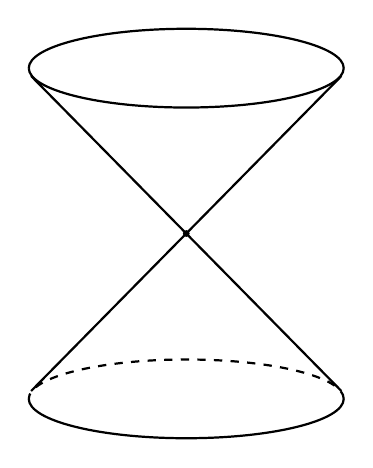
\begin{tikzpicture}
                \draw[thick] (2,0) arc (0:180:2 and 0.5);
                \draw[thick] (2,0) arc (0:-180:2 and 0.5);
                \draw[thick] (1.97,-4.1) -- (-1.97,-0.1);
                \draw[thick] (-1.97,-4.1) -- (1.97,-0.1);
                \draw[thick, dashed] (2,-4.2) arc (0:180:2 and 0.5);
                \draw[thick] (2,-4.2) arc (0:-180:2 and 0.5);
                \filldraw (0,-2.1) circle (1pt);
                \end{tikzpicture}
            \end{figure} 
            \noindent
            Como podemos ver de forma intuitiva, tenemos que el punto $(0,0,0)$ no tiene un entorno abierto homeomorfo a un abierto de $\mathbb{R}^2$. Formalmente, por reducción al absurdo, si existiera $U\subseteq S$ entorno abierto de $(0,0,0)$ homeomorfo a $V\subseteq \mathbb{R}^2$ abierto mediante un homeomorfismo $f:U\to V$, tendríamos entonces que $f:U\setminus\{(0,0,0)\} \to V\setminus\{f(0,0,0)\}$ sería un homeomorfismo, pero $U\setminus\{(0,0,0)\}$ no es conexo y $V\setminus\{f(0,0,0)\}$ sí sigue siendo conexo, hemos llegado a una contradicción.

        \item $\mathbb{R}^n$ con $n\neq 2$.

            Vemos que $\mathbb{R}$ no es una superficie, puesto que en caso de serlo podemos quitar un punto y por un argumento de conexión llegamos a contradicción.

            Para $\mathbb{R}^n$ con $n>2$, supongamos que sí es una superficie, con lo que para $0=(0,0,\ldots,0)\in \mathbb{R}^n$ podemos encontrar un entorno abierto suyo $U$ homeomorfo a un abierto $V$ de $\mathbb{R}^2$. Como $U$ es abierto existe $r$ de forma que $B(0,r)\subseteq U$, y su imagen será un subconjunto abierto simplemente conexo de $V$. De esta forma, tenemos que $B(0,r)\setminus\{0\}$ sigue siendo simplemente conexo (ya que un retracto de deformación suyo es $S(0,\nicefrac{r}{2})$, que sabemos que tiene grupo fundamental trivial por ser homeomorfa a $\mathbb{S}^{n-1}$ con $n>2$) pero su imagen por el homeomorfismo no, llegando a contradicción.
        \item $S = \{(x,y)\in \mathbb{R}^2 : y\geq 0\}$.

            Supuesto que $S$ tiene un entorno abierto homeomorfo a un abierto de $\mathbb{R}^2$, quitando un punto de la recta $y=0$ dentro de dicho entorno podemos llegar a contradicción, puesto que dentro del conjunto descrito puede encontrarse un disco abierto que contiene al punto, que menos el punto en $y=0$ sigue siendo simplemente conexo pero su imagen por el homeomorfismo no.
    \end{enumerate}
    ¿Es la unión o intersección de dos superficies en $\mathbb{R}^3$ una superficie?
    \begin{itemize}
        \item La unión de dos superficies no es una superficie, en $\mathbb{R}^3$ tenemos que las esferas $S((0,1),1)$ y $S((0,-1),1)$ son homeomorfas a $\mathbb{S}^2$ (y por tanto superficies), pero su unión no es una superficie, puede demostrarse con un argumento similar al que hicimos para el cono anteriormente.
        \item La intersección de dos superficientes tampoco es una superficie: en $\mathbb{R}^3$ tenemos que $\mathbb{R}^2\times \{0\}$ y $\mathbb{S}^2$ son superficies, pero su intersección es $\mathbb{S}^1\times \{0\}$, que no es una superficie.
    \end{itemize}
\end{ejercicio}

\begin{ejercicio}
    Sea $(R,p)$ un recubridor de una superficie topológica $S$. Si $R$ es 2AN, demuestra que $R$ es una superficie topológica.\\

    \noindent
    Sea $r\in R$ y $b = p(r)$, tenemos que existe un entorno abierto $O_b$ de $b$ regularmente recubierto por $p$, con lo que podemos obtener un abierto $A_r$ de $R$ que contiene a $r$ y de forma que $p\big|_{A_r}:A_r\to O_b$ es un homeomorfismo. Como $S$ es una superficie, $b$ admite un entorno abierto $V_b$ homeomorfo a un abierto de $\mathbb{R}^2$, por lo que el entorno abierto:
    \begin{equation*}
        W_b = V_b\cap O_b
    \end{equation*}
    será también homeomorfo a un abierto de $\mathbb{R}^2$, gracias a la restricción del homeomorfismo. Así, basta considerar el entorno $p\big|_{A_r}^{-1}(W_b)$ para obtener un entorno abierto de $r$ que es homeomorfo a un abierto de $\mathbb{R}^2$.\\

    \noindent
    Como $R$ es 2AN, basta ver que $R$ es T2 para probar que $R$ es una superficie. Sean $x,y\in R$ puntos distintos, tenemos que:
    \begin{itemize}
        \item Si $p(x) = p(y)$ entonces para este punto existe un abierto $O$ regularmente recubierto de forma que:
            \begin{equation*}
                p^{-1}(O) = \biguplus_{i \in I}A_i
            \end{equation*}
            con $A_i$ abierto y $p\big|_{A_i}:A_i\to O$ homeomorfismo, $\forall i \in I$. En dicho caso, tenemos que existen $j,k\in I$ de forma que $x\in A_j$, $y \in A_k$ y como $x\neq y$ y la unión es disjunta tenemos que $A_j$ y $A_k$ son dos abiertos disjuntos, hemos conseguido ``separar'' $x$ de $y$.
        \item Si $p(x) \neq p(y)$, como $S$ es T2 por ser una superficie tenemos que existen $O_x$, $O_y$ entornos abiertos disjuntos de $p(x)$ y de $p(y)$ de forma respectiva. Si consideramos los abiertos $p^{-1}(O_x)$ y $p^{-1}(O_y)$ tenemos entonces que estos son entornos abiertos de $O_x$ y de $O_y$ disjuntos, por lo que hemos ``separado'' $x$ de $y$.
    \end{itemize}
\end{ejercicio}

\begin{ejercicio}
    Sean $S$ una superficie y $f:S\to \mathbb{R}$ una función continua. Definimos el grafo de $f$ como el espacio topológico
    \begin{equation*}
        G(f) = \{(x,t)\in S\times \mathbb{R} : t=f(x)\}
    \end{equation*}
    con la topología inducida por la topología producto en $S\times \mathbb{R}$. Prueba que $G(f)$ es una superficie, que además es compacta si y solo si lo es $S$. % // TODO:
\end{ejercicio}

\begin{ejercicio}\label{ej:suma_chi}
    Prueba que la característica de Euler de la suma conexa de dos superficies compactas es igual a la suma de sus características de Euler menos dos.\\

    \noindent
    Sean $S_1$ y $S_2$ dos superficies compactas, podemos encontrar $\cc{P}_1$ y $\cc{P}_2$ presentaciones poligonales de forma respectiva de cada una de ellas con una expresión cada una, de forma que tengamos:
    \begin{gather*}
        C_1 = 1, \qquad A_1, \qquad V_1 \\
        C_2 = 1, \qquad A_2, \qquad V_2
    \end{gather*}
    Si hacemos la suma conexa de las superficies a través de un vértice, obtendremos que la superficie $S_1\# S_2$ tiene una presentación poligonal con:
    \begin{equation*}
        C = 1, \qquad A = A_1 + A_2, \qquad V = (V_1-1) + (V_2-1) + 1
    \end{equation*}
    Obtenemos así que:
    \begin{align*}
        \chi(S_1 \# S_2) &= V_1 + V_2 - 1 -A_1 - A_2 + 1 = V_1 - A_1 + V_2 - A_2 \\
        \chi(S_1) + \chi(S_2) - 2 &= V_1 - A_1 + 1 + V_2 - A_2 + 1 - 2 = V_1 - A_1 + V_2 - A_2
    \end{align*}
\end{ejercicio}

\begin{ejercicio}
    Calcula la característica de Euler de la suma conexa de un plano proyectivo y $n$ toros.\\

    \noindent
    A partir del ejercicio anterior tenemos que:
    \begin{equation*}
        \chi(\mathbb{R}\bb{P}^2 \# \mathbb{T}_n) = \chi(\mathbb{R}\bb{P}^2) + \chi(\mathbb{T}_n) - 2
    \end{equation*}
    Y sabemos que:
    \begin{equation*}
        \chi(\mathbb{R}\mathbb{P}^2) = 1, \qquad \chi(\mathbb{T}_n) = 2(n-1) \quad n\geq 1
    \end{equation*}
    Por lo que:
    \begin{equation*}
        \chi(\mathbb{R}\bb{P}^2 \# \mathbb{T}_n) = \chi(\mathbb{R}\bb{P}^2) + \chi(\mathbb{T}_n) - 2 = 1 + 2(n-1) - 2 = 2n -3
    \end{equation*}
\end{ejercicio}

\begin{ejercicio}\label{ej:orientabilidad}
    Estudia la orientabilidad de $S_1 \# S_2$ a partir de la de $S_1$ y de $S_2$.\\

    \noindent
    Podemos tomar $\cc{P}_1$ y $\cc{P}_2$ presentaciones poligonales para $S_1$ y $S_2$ de forma respectiva y de una expresión cada una, por lo que tendremos:
    \begin{align*}
        \cc{P}_1 &= \langle a_1,\ldots,a_n : w_1 \rangle  \\
        \cc{P}_2 &= \langle b_1,\ldots,b_m : w_2 \rangle
    \end{align*}
    Y en teoría hemos visto que una presentación poligonal para $S_1\# S_2$ es:
    \begin{equation*}
        \cc{P} = \langle a_1,\ldots,a_n,b_1,\ldots,b_m : w_1w_2 \rangle 
    \end{equation*}
    De esta forma:
    \begin{itemize}
        \item Si $S_1$ o $S_2$ es no orientable tenemos entonces que su correspondiente presentación poligonal es no orientada, es decir, que contiene dos letras del mismo exponente, por lo que $w_1w_2$  también contendrá dos letras del mismo exponente, por lo que $S_1\# S_2$ será no orientable.
        \item Si $S_1$ y $S_2$ son orientables tendremos que sus correspondientes presentaciones son orientadas, con lo que no aparece ni en $w_1$ ni en $w_2$ dos letras con el mismo exponente, por lo que en $w_1w_2$ tampoco, con lo que $S_1\# S_2$ es orientable.
    \end{itemize}
\end{ejercicio}

\begin{ejercicio}
    Para cada una de las siguientes presentaciones poligonales de superficies compactas, calcula la característica de Euler y determina a cuál de las superficies modelo es homeomorfa:\\

    \noindent
    Recordamos que las superficienes modelo son:
    \begin{equation*}
        \mathbb{S}^2, \qquad \mathbb{T}_n, \qquad \mathbb{R}\bb{P}^2_n
    \end{equation*}

    y tenemos que:
    \begin{equation*}
        \chi(\mathbb{S}^2) = 2, \qquad \chi(\bb{T}_n) = 2(1-n), \qquad \chi(\mathbb{R}\bb{P}^2_n) = 2-n; \qquad n\geq 1
    \end{equation*}
    \begin{enumerate}[label=\alph*)]
        \item $\langle a,b,c;abacb^{-1}c^{-1} \rangle $.

            Sea $|\cc{P}|$ su realización geométrica, tenemos que:
            \begin{equation*}
                \chi(|\cc{P}|) = V-A+C
            \end{equation*}
            Vemos que:
            \begin{itemize}
                \item $C = 1$, pues la presentación solo cuenta con una palabra.
                \item $A = 3$, pues la presentación cuenta con 3 símbolos.
            \end{itemize}
            Para el número de vértices, tenemos que observar la figura:
            \begin{figure}[H]
                \centering
                 \begin{tikzpicture}[
                    flechaCCW/.style={postaction={decorate}, decoration={markings, mark=at position 0.5 with {\arrow{Latex[length=3mm]}}}, thick},
                    flechaCW/.style={postaction={decorate}, decoration={markings, mark=at position 0.5 with {\arrow{Latex[length=3mm, reversed]}}}, thick},
                    etiqueta/.style={midway, auto, swap, font=\small}
                ]
                \def\R{1} % Radio del hexágono

                \foreach \i in {0,...,5} {
                    \pgfmathsetmacro{\angle}{\i * 60}
                    \coordinate (P\i) at (\angle:\R);
                }

                % Aristas en sentido antihorario
                \draw[flechaCCW] (P0) -- node[etiqueta] {$a$} (P1);
                \draw[flechaCCW] (P1) -- node[etiqueta] {$b$} (P2);
                \draw[flechaCCW] (P2) -- node[etiqueta] {$a$} (P3); 
                \draw[flechaCCW] (P3) -- node[etiqueta] {$c$} (P4);
                \draw[flechaCW] (P4) -- node[etiqueta] {$b^{-1}$} (P5);
                \draw[flechaCW] (P5) -- node[etiqueta] {$c^{-1}$} (P0);
            \end{tikzpicture}
            \end{figure}
            \noindent
            Analicemos sus vértices en el espacio topológico cociente:
            \begin{itemize}
                \item El vértice en el que empieza la arista $a$ de la derecha se pega con el vértice que empieza en la arista $a$ de la izquierda, que es el mismo vértice en el que termina $b$, que es el mismo vértice en el que termina $c$, que es el mismo vértice en el que empieza $b$, que es el mismo vértice en el que termina $a$, que es el mismo vértice en el que empieza $c$, que es el mismo vértice en el que empieza $a$.

                    Hemos cerrado el ciclo, por lo que todos estos vértices se identifican en el cociente.
            \end{itemize}
            Hemos dejado al polígono sin vértices, por lo que todos estos son iguales en el cociente:
            \begin{figure}[H]
                \centering
                 \begin{tikzpicture}[
                    flechaCCW/.style={postaction={decorate}, decoration={markings, mark=at position 0.5 with {\arrow{Latex[length=3mm]}}}, thick},
                    flechaCW/.style={postaction={decorate}, decoration={markings, mark=at position 0.5 with {\arrow{Latex[length=3mm, reversed]}}}, thick},
                    etiqueta/.style={midway, auto, swap, font=\small}
                ]
                \def\R{1} % Radio del hexágono

                \foreach \i in {0,...,5} {
                    \pgfmathsetmacro{\angle}{\i * 60}
                    \coordinate (P\i) at (\angle:\R);
                }

                % Aristas en sentido antihorario
                \draw[flechaCCW] (P0) -- node[etiqueta] {$a$} (P1);
                \draw[flechaCCW] (P1) -- node[etiqueta] {$b$} (P2);
                \draw[flechaCCW] (P2) -- node[etiqueta] {$a$} (P3); 
                \draw[flechaCCW] (P3) -- node[etiqueta] {$c$} (P4);
                \draw[flechaCW] (P4) -- node[etiqueta] {$b^{-1}$} (P5);
                \draw[flechaCW] (P5) -- node[etiqueta] {$c^{-1}$} (P0);

                % Colores de los vértices
                \filldraw[fill=yellow, draw=black] (P0) circle (2pt);
                \filldraw[fill=yellow, draw=black] (P1) circle (2pt);
                \filldraw[fill=yellow, draw=black] (P2) circle (2pt);
                \filldraw[fill=yellow, draw=black] (P3) circle (2pt);
                \filldraw[fill=yellow, draw=black] (P4) circle (2pt);
                \filldraw[fill=yellow, draw=black] (P5) circle (2pt);
            \end{tikzpicture}
            \end{figure}
            \noindent
            Tenemos así que $V = 1$, por lo que:
            \begin{equation*}
                \chi(|\cc{P}|) = V-A+C = 1-3+1 = -1
            \end{equation*}
            Vemos que obtenemos un número negativo e impar, por lo que tiene que ser el producto de un plano proyectivo consigo mismo $n$ veces, y como:
            \begin{equation*}
                \chi(\mathbb{R}\mathbb{P}^2_n) = 2-n
            \end{equation*}
            vemos entonces que $n=3$, es decir:
            \begin{equation*}
                |\cc{P}| \cong \mathbb{R}\bb{P}^2_3
            \end{equation*}
        \item $\langle a,b,c;abca^{-1}b^{-1}c^{-1} \rangle $.

            Sea $|\cc{P}|$ su realización geométrica, tenemos que:
            \begin{itemize}
                \item $C = 1$.
                \item $A = 3$.
            \end{itemize}
            Para los vértices, vemos que tenemos la figura:
            \begin{figure}[H]
                \centering
                 \begin{tikzpicture}[
                    flechaCCW/.style={postaction={decorate}, decoration={markings, mark=at position 0.5 with {\arrow{Latex[length=3mm]}}}, thick},
                    flechaCW/.style={postaction={decorate}, decoration={markings, mark=at position 0.5 with {\arrow{Latex[length=3mm, reversed]}}}, thick},
                    etiqueta/.style={midway, auto, swap, font=\small}
                ]
                \def\R{1} % Radio del hexágono

                \foreach \i in {0,...,5} {
                    \pgfmathsetmacro{\angle}{\i * 60}
                    \coordinate (P\i) at (\angle:\R);
                }

                % Aristas en sentido antihorario
                \draw[flechaCCW] (P0) -- node[etiqueta] {$a$} (P1);
                \draw[flechaCCW] (P1) -- node[etiqueta] {$b$} (P2);
                \draw[flechaCCW] (P2) -- node[etiqueta] {$c$} (P3); 
                \draw[flechaCW] (P3) -- node[etiqueta] {$a^{-1}$} (P4);
                \draw[flechaCW] (P4) -- node[etiqueta] {$b^{-1}$} (P5);
                \draw[flechaCW] (P5) -- node[etiqueta] {$c^{-1}$} (P0);
            \end{tikzpicture}
            \end{figure}
            \noindent
            Contamos sus vértices:
            \begin{itemize}
                \item El vértice en el que empieza $a$ también es el vértice en el que termina $b$, que también es el vértice en el que empieza $c$, que es el vértice en el que empieza $a$. Hemos cerrado el ciclo.
                \item El vértice en el que termina $a$ es también donde termina $c$, que es donde comienza $b$ y donde termina $a$. Hemos cerrado el ciclo.
            \end{itemize}
            Hemos obtenido así $2$ vértices:
            \begin{figure}[H]
                \centering
                 \begin{tikzpicture}[
                    flechaCCW/.style={postaction={decorate}, decoration={markings, mark=at position 0.5 with {\arrow{Latex[length=3mm]}}}, thick},
                    flechaCW/.style={postaction={decorate}, decoration={markings, mark=at position 0.5 with {\arrow{Latex[length=3mm, reversed]}}}, thick},
                    etiqueta/.style={midway, auto, swap, font=\small}
                ]
                \def\R{1} % Radio del hexágono

                \foreach \i in {0,...,5} {
                    \pgfmathsetmacro{\angle}{\i * 60}
                    \coordinate (P\i) at (\angle:\R);
                }

                % Aristas en sentido antihorario
                \draw[flechaCCW] (P0) -- node[etiqueta] {$a$} (P1);
                \draw[flechaCCW] (P1) -- node[etiqueta] {$b$} (P2);
                \draw[flechaCCW] (P2) -- node[etiqueta] {$c$} (P3); 
                \draw[flechaCW] (P3) -- node[etiqueta] {$a^{-1}$} (P4);
                \draw[flechaCW] (P4) -- node[etiqueta] {$b^{-1}$} (P5);
                \draw[flechaCW] (P5) -- node[etiqueta] {$c^{-1}$} (P0);

                % Colores de los vértices
                \filldraw[fill=yellow, draw=black] (P0) circle (2pt);
                \filldraw[fill=red, draw=black] (P1) circle (2pt);
                \filldraw[fill=yellow, draw=black] (P2) circle (2pt);
                \filldraw[fill=red, draw=black] (P3) circle (2pt);
                \filldraw[fill=yellow, draw=black] (P4) circle (2pt);
                \filldraw[fill=red, draw=black] (P5) circle (2pt);
            \end{tikzpicture}
            \end{figure}
            \noindent
            Tenemos entonces que:
            \begin{equation*}
                \chi(|\cc{P}|) = V-A+C = 2-3+1 = 0
            \end{equation*}
            Por lo que nuestra superficie $|\cc{P}|$ puede ser $\bb{T}$ o $\mathbb{R}\bb{P}^2_2$. Vemos que la presentación poligonal es orientada, por lo que la superficie $|\cc{P}|$ es orientable, luego ha de ser:
            \begin{equation*}
                |\cc{P}| \cong \mathbb{T}
            \end{equation*}
        \item $\langle a,b,c,d;abcdca^{-1}bd^{-1} \rangle $.

            Sea $|\cc{P}|$ la realización geométrica de la presentación, tenemos:
            \begin{itemize}
                \item $C=1$.
                \item $A=4$.
            \end{itemize}
            Tenemos el polígono:
            \begin{figure}[H]
                \centering
                 \begin{tikzpicture}[
                    flechaCCW/.style={postaction={decorate}, decoration={markings, mark=at position 0.7 with {\arrow{Latex[length=3mm]}}}, thick},
                    flechaCW/.style={postaction={decorate}, decoration={markings, mark=at position 0.7 with {\arrow{Latex[length=3mm, reversed]}}}, thick},
                    etiqueta/.style={midway, auto, swap, font=\small}
                ]
                \def\R{1} % Radio del hexágono

                \foreach \i in {0,...,7} {
                    \pgfmathsetmacro{\angle}{\i * 45}
                    \coordinate (P\i) at (\angle:\R);
                }

                % Aristas en sentido antihorario
                \draw[flechaCCW] (P0) -- node[etiqueta] {$a$} (P1);
                \draw[flechaCCW] (P1) -- node[etiqueta] {$b$} (P2);
                \draw[flechaCCW] (P2) -- node[etiqueta] {$c$} (P3); 
                \draw[flechaCCW] (P3) -- node[etiqueta] {$d$} (P4);
                \draw[flechaCCW] (P4) -- node[etiqueta] {$c$} (P5);
                \draw[flechaCW] (P5) -- node[etiqueta] {$a^{-1}$} (P6);
                \draw[flechaCCW] (P6) -- node[etiqueta] {$b$} (P7);
                \draw[flechaCW] (P7) -- node[etiqueta] {$d^{-1}$} (P0);

%                 % Colores de los vértices
%                 \filldraw[fill=yellow, draw=black] (P0) circle (2pt);
%                 \filldraw[fill=yellow, draw=black] (P1) circle (2pt);
%                 \filldraw[fill=yellow, draw=black] (P2) circle (2pt);
%                 \filldraw[fill=yellow, draw=black] (P3) circle (2pt);
%                 \filldraw[fill=yellow, draw=black] (P4) circle (2pt);
%                 \filldraw[fill=yellow, draw=black] (P5) circle (2pt);
            \end{tikzpicture}
            \end{figure}
            \noindent
            Y si calculamos sus vértices obtendremos:
            \begin{equation*}
                V = 2
            \end{equation*}
            ya que:
            \begin{figure}[H]
                \centering
                 \begin{tikzpicture}[
                    flechaCCW/.style={postaction={decorate}, decoration={markings, mark=at position 0.7 with {\arrow{Latex[length=3mm]}}}, thick},
                    flechaCW/.style={postaction={decorate}, decoration={markings, mark=at position 0.7 with {\arrow{Latex[length=3mm, reversed]}}}, thick},
                    etiqueta/.style={midway, auto, swap, font=\small}
                ]
                \def\R{1} % Radio del hexágono

                \foreach \i in {0,...,7} {
                    \pgfmathsetmacro{\angle}{\i * 45}
                    \coordinate (P\i) at (\angle:\R);
                }

                % Aristas en sentido antihorario
                \draw[flechaCCW] (P0) -- node[etiqueta] {$a$} (P1);
                \draw[flechaCCW] (P1) -- node[etiqueta] {$b$} (P2);
                \draw[flechaCCW] (P2) -- node[etiqueta] {$c$} (P3); 
                \draw[flechaCCW] (P3) -- node[etiqueta] {$d$} (P4);
                \draw[flechaCCW] (P4) -- node[etiqueta] {$c$} (P5);
                \draw[flechaCW] (P5) -- node[etiqueta] {$a^{-1}$} (P6);
                \draw[flechaCCW] (P6) -- node[etiqueta] {$b$} (P7);
                \draw[flechaCW] (P7) -- node[etiqueta] {$d^{-1}$} (P0);

                % Colores de los vértices
                \filldraw[fill=yellow, draw=black] (P0) circle (2pt);
                \filldraw[fill=yellow, draw=black] (P1) circle (2pt);
                \filldraw[fill=red, draw=black] (P2) circle (2pt);
                \filldraw[fill=yellow, draw=black] (P3) circle (2pt);
                \filldraw[fill=red, draw=black] (P4) circle (2pt);
                \filldraw[fill=yellow, draw=black] (P5) circle (2pt);
                \filldraw[fill=yellow, draw=black] (P6) circle (2pt);
                \filldraw[fill=red, draw=black] (P7) circle (2pt);
            \end{tikzpicture}
            \end{figure}
            \noindent
            Tenemos así que:
            \begin{equation*}
                \chi(|\cc{P}|) = 2-4+1 = -1
            \end{equation*}
            Por lo que:
            \begin{equation*}
                |\cc{P}|\cong \mathbb{R}\bb{P}^2_3
            \end{equation*}
        \item $\langle a,b,c,d,e;aba^{-1}cdb^{-1}c^{-1}ed^{-1}e^{-1} \rangle $.
            Sea $|\cc{P}|$ su realización geométrica, tenemos que:
            \begin{itemize}
                \item $C=1$.
                \item $A=5$
            \end{itemize}
            El polígono es:
            \begin{figure}[H]
                \centering
                 \begin{tikzpicture}[
                    flechaCCW/.style={postaction={decorate}, decoration={markings, mark=at position 0.7 with {\arrow{Latex[length=3mm]}}}, thick},
                    flechaCW/.style={postaction={decorate}, decoration={markings, mark=at position 0.7 with {\arrow{Latex[length=3mm, reversed]}}}, thick},
                    etiqueta/.style={midway, auto, swap, font=\small}
                ]
                \def\R{1.5} % Radio del hexágono

                \foreach \i in {0,...,9} {
                    \pgfmathsetmacro{\angle}{\i * 36}
                    \coordinate (P\i) at (\angle:\R);
                }

                % Aristas en sentido antihorario
                \draw[flechaCCW] (P0) -- node[etiqueta] {$a$} (P1);
                \draw[flechaCCW] (P1) -- node[etiqueta] {$b$} (P2);
                \draw[flechaCW] (P2) -- node[etiqueta] {$a^{-1}$} (P3); 
                \draw[flechaCCW] (P3) -- node[etiqueta] {$c$} (P4);
                \draw[flechaCCW] (P4) -- node[etiqueta] {$d$} (P5);
                \draw[flechaCW] (P5) -- node[etiqueta] {$b^{-1}$} (P6);
                \draw[flechaCW] (P6) -- node[etiqueta] {$c^{-1}$} (P7);
                \draw[flechaCCW] (P7) -- node[etiqueta] {$e$} (P8);
                \draw[flechaCW] (P8) -- node[etiqueta] {$d^{-1}$} (P9);
                \draw[flechaCW] (P9) -- node[etiqueta] {$e^{-1}$} (P0);
            \end{tikzpicture}
            \end{figure}
            \noindent
            Y tenemos que:
            \begin{equation*}
                V = 2
            \end{equation*}
            ya que:
            \begin{figure}[H]
                \centering
                 \begin{tikzpicture}[
                    flechaCCW/.style={postaction={decorate}, decoration={markings, mark=at position 0.7 with {\arrow{Latex[length=3mm]}}}, thick},
                    flechaCW/.style={postaction={decorate}, decoration={markings, mark=at position 0.7 with {\arrow{Latex[length=3mm, reversed]}}}, thick},
                    etiqueta/.style={midway, auto, swap, font=\small}
                ]
                \def\R{1.5} % Radio del hexágono

                \foreach \i in {0,...,9} {
                    \pgfmathsetmacro{\angle}{\i * 36}
                    \coordinate (P\i) at (\angle:\R);
                }

                % Aristas en sentido antihorario
                \draw[flechaCCW] (P0) -- node[etiqueta] {$a$} (P1);
                \draw[flechaCCW] (P1) -- node[etiqueta] {$b$} (P2);
                \draw[flechaCW] (P2) -- node[etiqueta] {$a^{-1}$} (P3); 
                \draw[flechaCCW] (P3) -- node[etiqueta] {$c$} (P4);
                \draw[flechaCCW] (P4) -- node[etiqueta] {$d$} (P5);
                \draw[flechaCW] (P5) -- node[etiqueta] {$b^{-1}$} (P6);
                \draw[flechaCW] (P6) -- node[etiqueta] {$c^{-1}$} (P7);
                \draw[flechaCCW] (P7) -- node[etiqueta] {$e$} (P8);
                \draw[flechaCW] (P8) -- node[etiqueta] {$d^{-1}$} (P9);
                \draw[flechaCW] (P9) -- node[etiqueta] {$e^{-1}$} (P0);

                % Colores de los vértices
                \filldraw[fill=yellow, draw=black] (P0) circle (2pt);
                \filldraw[fill=red, draw=black] (P1) circle (2pt);
                \filldraw[fill=red, draw=black] (P2) circle (2pt);
                \filldraw[fill=yellow, draw=black] (P3) circle (2pt);
                \filldraw[fill=red, draw=black] (P4) circle (2pt);
                \filldraw[fill=red, draw=black] (P5) circle (2pt);
                \filldraw[fill=red, draw=black] (P6) circle (2pt);
                \filldraw[fill=yellow, draw=black] (P7) circle (2pt);
                \filldraw[fill=red, draw=black] (P8) circle (2pt);
                \filldraw[fill=red, draw=black] (P9) circle (2pt);
            \end{tikzpicture}
            \end{figure}
            \noindent
            En definitiva:
            \begin{equation*}
                \chi(|\cc{P}|) = 2-5+1 = -2
            \end{equation*}
            Por lo que puede ser $\mathbb{T}_2$ o $\mathbb{R}\bb{P}^2_4$. Vemos que la presentación es orientada, por lo que $|\cc{P}|$ es orientable, de donde tiene que ser:
            \begin{equation*}
                |\cc{P}| \cong \mathbb{T}_2
            \end{equation*}

        \item $\langle a,b,c,d,e,f;abcadb^{-1}efce^{-1}df^{-1} \rangle $.
            Sea $|\cc{P}|$ su realización geométrica, tenemos que:
            \begin{itemize}
                \item $C=1$.
                \item $A=6$
            \end{itemize}
            El polígono es:
            \begin{figure}[H]
                \centering
                 \begin{tikzpicture}[
                    flechaCCW/.style={postaction={decorate}, decoration={markings, mark=at position 0.7 with {\arrow{Latex[length=3mm]}}}, thick},
                    flechaCW/.style={postaction={decorate}, decoration={markings, mark=at position 0.7 with {\arrow{Latex[length=3mm, reversed]}}}, thick},
                    etiqueta/.style={midway, auto, swap, font=\small}
                ]
                \def\R{1.5} % Radio del hexágono

                \foreach \i in {0,...,11} {
                    \pgfmathsetmacro{\angle}{\i * 30}
                    \coordinate (P\i) at (\angle:\R);
                }

                % Aristas en sentido antihorario
                \draw[flechaCCW] (P0) -- node[etiqueta] {$a$} (P1);
                \draw[flechaCCW] (P1) -- node[etiqueta] {$b$} (P2);
                \draw[flechaCCW] (P2) -- node[etiqueta] {$c$} (P3); 
                \draw[flechaCCW] (P3) -- node[etiqueta] {$a$} (P4);
                \draw[flechaCCW] (P4) -- node[etiqueta] {$d$} (P5);
                \draw[flechaCW] (P5) -- node[etiqueta] {$b^{-1}$} (P6);
                \draw[flechaCCW] (P6) -- node[etiqueta] {$e$} (P7);
                \draw[flechaCCW] (P7) -- node[etiqueta] {$f$} (P8);
                \draw[flechaCCW] (P8) -- node[etiqueta] {$c$} (P9);
                \draw[flechaCW] (P9) -- node[etiqueta] {$e^{-1}$} (P10);
                \draw[flechaCCW] (P10) -- node[etiqueta] {$d$} (P11);
                \draw[flechaCW] (P11) -- node[etiqueta] {$f^{-1}$} (P0);
            \end{tikzpicture}
            \end{figure}
            \noindent
            Y tenemos que:
            \begin{equation*}
                V =3
            \end{equation*}
            ya que:
            \begin{figure}[H]
                \centering
                 \begin{tikzpicture}[
                    flechaCCW/.style={postaction={decorate}, decoration={markings, mark=at position 0.7 with {\arrow{Latex[length=3mm]}}}, thick},
                    flechaCW/.style={postaction={decorate}, decoration={markings, mark=at position 0.7 with {\arrow{Latex[length=3mm, reversed]}}}, thick},
                    etiqueta/.style={midway, auto, swap, font=\small}
                ]
                \def\R{1.5} % Radio del hexágono

                \foreach \i in {0,...,11} {
                    \pgfmathsetmacro{\angle}{\i * 30}
                    \coordinate (P\i) at (\angle:\R);
                }

                % Aristas en sentido antihorario
                \draw[flechaCCW] (P0) -- node[etiqueta] {$a$} (P1);
                \draw[flechaCCW] (P1) -- node[etiqueta] {$b$} (P2);
                \draw[flechaCCW] (P2) -- node[etiqueta] {$c$} (P3); 
                \draw[flechaCCW] (P3) -- node[etiqueta] {$a$} (P4);
                \draw[flechaCCW] (P4) -- node[etiqueta] {$d$} (P5);
                \draw[flechaCW] (P5) -- node[etiqueta] {$b^{-1}$} (P6);
                \draw[flechaCCW] (P6) -- node[etiqueta] {$e$} (P7);
                \draw[flechaCCW] (P7) -- node[etiqueta] {$f$} (P8);
                \draw[flechaCCW] (P8) -- node[etiqueta] {$c$} (P9);
                \draw[flechaCW] (P9) -- node[etiqueta] {$e^{-1}$} (P10);
                \draw[flechaCCW] (P10) -- node[etiqueta] {$d$} (P11);
                \draw[flechaCW] (P11) -- node[etiqueta] {$f^{-1}$} (P0);

                % Colores de los vértices
                \filldraw[fill=yellow, draw=black] (P0) circle (2pt);
                \filldraw[fill=red, draw=black] (P1) circle (2pt);
                \filldraw[fill=blue, draw=black] (P2) circle (2pt);
                \filldraw[fill=yellow, draw=black] (P3) circle (2pt);
                \filldraw[fill=red, draw=black] (P4) circle (2pt);
                \filldraw[fill=blue, draw=black] (P5) circle (2pt);
                \filldraw[fill=red, draw=black] (P6) circle (2pt);
                \filldraw[fill=yellow, draw=black] (P7) circle (2pt);
                \filldraw[fill=blue, draw=black] (P8) circle (2pt);
                \filldraw[fill=yellow, draw=black] (P9) circle (2pt);
                \filldraw[fill=red, draw=black] (P10) circle (2pt);
                \filldraw[fill=blue, draw=black] (P11) circle (2pt);
            \end{tikzpicture}
            \end{figure}
            \noindent
            Tenemos así que:
            \begin{equation*}
                \chi(|\cc{P}|) = 3-6+1 = -2
            \end{equation*}
            Por lo que puede ser $\mathbb{T}_2$ o $\mathbb{R}\bb{P}^2_4$. Vemos que la presentación es no orientada, por lo que $|\cc{P}|$ es no orientable, de donde será:
            \begin{equation*}
                |\cc{P}| \cong \mathbb{R}\bb{P}^2_4
            \end{equation*}

        \item $\langle a,b,c,d,e,f;abc,bde,c^{-1} d f, e^{-1}fa \rangle $.
            Sea $|\cc{P}|$ la realización geométrica de la presentación, tenemos en este caso que:
            \begin{itemize}
                \item $C=4$, ya que contamos con 4 expresiones.
                \item $A=6$.
            \end{itemize}
            Tenemos en este caso los polígonos:
            \begin{figure}[H]
                \centering
                \begin{minipage}{0.24\textwidth}
                    \centering
                     \begin{tikzpicture}[
                        flechaCCW/.style={postaction={decorate}, decoration={markings, mark=at position 0.7 with {\arrow{Latex[length=3mm]}}}, thick},
                        flechaCW/.style={postaction={decorate}, decoration={markings, mark=at position 0.7 with {\arrow{Latex[length=3mm, reversed]}}}, thick},
                        etiqueta/.style={midway, auto, swap, font=\small}
                    ]
                    \def\R{0.5} % Radio del hexágono

                    \foreach \i in {0,...,2} {
                        \pgfmathsetmacro{\angle}{\i * 120}
                        \coordinate (P\i) at (\angle:\R);
                    }

                    % Aristas en sentido antihorario
                    \draw[flechaCCW] (P0) -- node[etiqueta] {$a$} (P1);
                    \draw[flechaCCW] (P1) -- node[etiqueta] {$b$} (P2);
                    \draw[flechaCCW] (P2) -- node[etiqueta] {$c$} (P0); 
                \end{tikzpicture}
                \end{minipage}\hfill
                \begin{minipage}{0.24\textwidth}
                    
                    \centering
                     \begin{tikzpicture}[
                        flechaCCW/.style={postaction={decorate}, decoration={markings, mark=at position 0.7 with {\arrow{Latex[length=3mm]}}}, thick},
                        flechaCW/.style={postaction={decorate}, decoration={markings, mark=at position 0.7 with {\arrow{Latex[length=3mm, reversed]}}}, thick},
                        etiqueta/.style={midway, auto, swap, font=\small}
                    ]
                    \def\R{0.5} % Radio del hexágono

                    \foreach \i in {0,...,2} {
                        \pgfmathsetmacro{\angle}{\i * 120}
                        \coordinate (P\i) at (\angle:\R);
                    }

                    % Aristas en sentido antihorario
                    \draw[flechaCCW] (P0) -- node[etiqueta] {$b$} (P1);
                    \draw[flechaCCW] (P1) -- node[etiqueta] {$d$} (P2);
                    \draw[flechaCCW] (P2) -- node[etiqueta] {$e$} (P0); 
                \end{tikzpicture}
                \end{minipage}\hfill
                \begin{minipage}{0.24\textwidth}
                    
                    \centering
                     \begin{tikzpicture}[
                        flechaCCW/.style={postaction={decorate}, decoration={markings, mark=at position 0.7 with {\arrow{Latex[length=3mm]}}}, thick},
                        flechaCW/.style={postaction={decorate}, decoration={markings, mark=at position 0.7 with {\arrow{Latex[length=3mm, reversed]}}}, thick},
                        etiqueta/.style={midway, auto, swap, font=\small}
                    ]
                    \def\R{0.5} % Radio del hexágono

                    \foreach \i in {0,...,2} {
                        \pgfmathsetmacro{\angle}{\i * 120}
                        \coordinate (P\i) at (\angle:\R);
                    }

                    % Aristas en sentido antihorario
                    \draw[flechaCW] (P0) -- node[etiqueta] {$c^{-1}$} (P1);
                    \draw[flechaCCW] (P1) -- node[etiqueta] {$d$} (P2);
                    \draw[flechaCCW] (P2) -- node[etiqueta] {$f$} (P0); 
                \end{tikzpicture}
                \end{minipage}\hfill
                \begin{minipage}{0.24\textwidth}
                    
                    \centering
                     \begin{tikzpicture}[
                        flechaCCW/.style={postaction={decorate}, decoration={markings, mark=at position 0.7 with {\arrow{Latex[length=3mm]}}}, thick},
                        flechaCW/.style={postaction={decorate}, decoration={markings, mark=at position 0.7 with {\arrow{Latex[length=3mm, reversed]}}}, thick},
                        etiqueta/.style={midway, auto, swap, font=\small}
                    ]
                    \def\R{0.5} % Radio del hexágono

                    \foreach \i in {0,...,2} {
                        \pgfmathsetmacro{\angle}{\i * 120}
                        \coordinate (P\i) at (\angle:\R);
                    }

                    % Aristas en sentido antihorario
                    \draw[flechaCW] (P0) -- node[etiqueta] {$e^{-1}$} (P1);
                    \draw[flechaCCW] (P1) -- node[etiqueta] {$f$} (P2);
                    \draw[flechaCCW] (P2) -- node[etiqueta] {$a$} (P0); 
                \end{tikzpicture}
                \end{minipage}
            \end{figure}
            \noindent
            Y tenemos que:
            \begin{equation*}
                V = 4
            \end{equation*}
            ya que:
            \begin{figure}[H]
                \centering
                \begin{minipage}{0.24\textwidth}
                    \centering
                     \begin{tikzpicture}[
                        flechaCCW/.style={postaction={decorate}, decoration={markings, mark=at position 0.7 with {\arrow{Latex[length=3mm]}}}, thick},
                        flechaCW/.style={postaction={decorate}, decoration={markings, mark=at position 0.7 with {\arrow{Latex[length=3mm, reversed]}}}, thick},
                        etiqueta/.style={midway, auto, swap, font=\small}
                    ]
                    \def\R{0.5} % Radio del hexágono

                    \foreach \i in {0,...,2} {
                        \pgfmathsetmacro{\angle}{\i * 120}
                        \coordinate (P\i) at (\angle:\R);
                    }

                    % Aristas en sentido antihorario
                    \draw[flechaCCW] (P0) -- node[etiqueta] {$a$} (P1);
                    \draw[flechaCCW] (P1) -- node[etiqueta] {$b$} (P2);
                    \draw[flechaCCW] (P2) -- node[etiqueta] {$c$} (P0); 

                    % Colores de los vértices
                    \filldraw[fill=yellow, draw=black] (P0) circle (2pt);
                    \filldraw[fill=red, draw=black] (P1) circle (2pt);
                    \filldraw[fill=blue, draw=black] (P2) circle (2pt);
                \end{tikzpicture}
                \end{minipage}\hfill
                \begin{minipage}{0.24\textwidth}
                    
                    \centering
                     \begin{tikzpicture}[
                        flechaCCW/.style={postaction={decorate}, decoration={markings, mark=at position 0.7 with {\arrow{Latex[length=3mm]}}}, thick},
                        flechaCW/.style={postaction={decorate}, decoration={markings, mark=at position 0.7 with {\arrow{Latex[length=3mm, reversed]}}}, thick},
                        etiqueta/.style={midway, auto, swap, font=\small}
                    ]
                    \def\R{0.5} % Radio del hexágono

                    \foreach \i in {0,...,2} {
                        \pgfmathsetmacro{\angle}{\i * 120}
                        \coordinate (P\i) at (\angle:\R);
                    }

                    % Aristas en sentido antihorario
                    \draw[flechaCCW] (P0) -- node[etiqueta] {$b$} (P1);
                    \draw[flechaCCW] (P1) -- node[etiqueta] {$d$} (P2);
                    \draw[flechaCCW] (P2) -- node[etiqueta] {$e$} (P0); 

                    % Colores de los vértices
                    \filldraw[fill=red, draw=black] (P0) circle (2pt);
                    \filldraw[fill=blue, draw=black] (P1) circle (2pt);
                    \filldraw[fill=green, draw=black] (P2) circle (2pt);
                \end{tikzpicture}
                \end{minipage}\hfill
                \begin{minipage}{0.24\textwidth}
                    
                    \centering
                     \begin{tikzpicture}[
                        flechaCCW/.style={postaction={decorate}, decoration={markings, mark=at position 0.7 with {\arrow{Latex[length=3mm]}}}, thick},
                        flechaCW/.style={postaction={decorate}, decoration={markings, mark=at position 0.7 with {\arrow{Latex[length=3mm, reversed]}}}, thick},
                        etiqueta/.style={midway, auto, swap, font=\small}
                    ]
                    \def\R{0.5} % Radio del hexágono

                    \foreach \i in {0,...,2} {
                        \pgfmathsetmacro{\angle}{\i * 120}
                        \coordinate (P\i) at (\angle:\R);
                    }

                    % Aristas en sentido antihorario
                    \draw[flechaCW] (P0) -- node[etiqueta] {$c^{-1}$} (P1);
                    \draw[flechaCCW] (P1) -- node[etiqueta] {$d$} (P2);
                    \draw[flechaCCW] (P2) -- node[etiqueta] {$f$} (P0); 

                    % Colores de los vértices
                    \filldraw[fill=yellow, draw=black] (P0) circle (2pt);
                    \filldraw[fill=blue, draw=black] (P1) circle (2pt);
                    \filldraw[fill=green, draw=black] (P2) circle (2pt);
                \end{tikzpicture}
                \end{minipage}\hfill
                \begin{minipage}{0.24\textwidth}
                    
                    \centering
                     \begin{tikzpicture}[
                        flechaCCW/.style={postaction={decorate}, decoration={markings, mark=at position 0.7 with {\arrow{Latex[length=3mm]}}}, thick},
                        flechaCW/.style={postaction={decorate}, decoration={markings, mark=at position 0.7 with {\arrow{Latex[length=3mm, reversed]}}}, thick},
                        etiqueta/.style={midway, auto, swap, font=\small}
                    ]
                    \def\R{0.5} % Radio del hexágono

                    \foreach \i in {0,...,2} {
                        \pgfmathsetmacro{\angle}{\i * 120}
                        \coordinate (P\i) at (\angle:\R);
                    }

                    % Aristas en sentido antihorario
                    \draw[flechaCW] (P0) -- node[etiqueta] {$e^{-1}$} (P1);
                    \draw[flechaCCW] (P1) -- node[etiqueta] {$f$} (P2);
                    \draw[flechaCCW] (P2) -- node[etiqueta] {$a$} (P0); 

                    % Colores de los vértices
                    \filldraw[fill=red, draw=black] (P0) circle (2pt);
                    \filldraw[fill=green, draw=black] (P1) circle (2pt);
                    \filldraw[fill=yellow, draw=black] (P2) circle (2pt);
                \end{tikzpicture}
                \end{minipage}
            \end{figure}
            \noindent
            Por lo que:
            \begin{equation*}
                \chi(|\cc{P}|) = 4-6+4 = 2
            \end{equation*}
            Y la única posibilidad es $|\cc{P}|\cong \mathbb{S}^2$.
        \item $\langle a,b,c,d,e,f,g,h,i,j,k,l,m,n,o;\\ abc, bde,dfg, fhi, haj, c^{-1}kl, e^{-1}mn, g^{-1}ok^{-1}, i^{-1}l^{-1}m^{-1}, j^{-1}n^{-1}o^{-1} \rangle $. 

            Tenemos que:
            \begin{itemize}
                \item $C = 10$.
                \item $A = 15$.
            \end{itemize}
            Los polígonos que tenemos son:
            \begin{figure}[H]
                \centering
                \begin{minipage}{0.24\textwidth}
                    \centering
                     \begin{tikzpicture}[
                        flechaCCW/.style={postaction={decorate}, decoration={markings, mark=at position 0.7 with {\arrow{Latex[length=3mm]}}}, thick},
                        flechaCW/.style={postaction={decorate}, decoration={markings, mark=at position 0.7 with {\arrow{Latex[length=3mm, reversed]}}}, thick},
                        etiqueta/.style={midway, auto, swap, font=\small}
                    ]
                    \def\R{0.5} % Radio del hexágono

                    \foreach \i in {0,...,2} {
                        \pgfmathsetmacro{\angle}{\i * 120}
                        \coordinate (P\i) at (\angle:\R);
                    }

                    % Aristas en sentido antihorario
                    \draw[flechaCCW] (P0) -- node[etiqueta] {$a$} (P1);
                    \draw[flechaCCW] (P1) -- node[etiqueta] {$b$} (P2);
                    \draw[flechaCCW] (P2) -- node[etiqueta] {$c$} (P0); 
                \end{tikzpicture}
                \end{minipage}\hfill
                \begin{minipage}{0.24\textwidth}
                    
                    \centering
                    \begin{tikzpicture}[
                        flechaCCW/.style={postaction={decorate}, decoration={markings, mark=at position 0.7 with {\arrow{Latex[length=3mm]}}}, thick},
                        flechaCW/.style={postaction={decorate}, decoration={markings, mark=at position 0.7 with {\arrow{Latex[length=3mm, reversed]}}}, thick},
                        etiqueta/.style={midway, auto, swap, font=\small}
                    ]
                    \def\R{0.5} % Radio del hexágono

                    \foreach \i in {0,...,2} {
                        \pgfmathsetmacro{\angle}{\i * 120}
                        \coordinate (P\i) at (\angle:\R);
                    }

                    % Aristas en sentido antihorario
                    \draw[flechaCCW] (P0) -- node[etiqueta] {$b$} (P1);
                    \draw[flechaCCW] (P1) -- node[etiqueta] {$d$} (P2);
                    \draw[flechaCCW] (P2) -- node[etiqueta] {$e$} (P0); 
                \end{tikzpicture}
                \end{minipage}\hfill
                \begin{minipage}{0.24\textwidth}
                    
                    \centering
                    \begin{tikzpicture}[
                        flechaCCW/.style={postaction={decorate}, decoration={markings, mark=at position 0.7 with {\arrow{Latex[length=3mm]}}}, thick},
                        flechaCW/.style={postaction={decorate}, decoration={markings, mark=at position 0.7 with {\arrow{Latex[length=3mm, reversed]}}}, thick},
                        etiqueta/.style={midway, auto, swap, font=\small}
                    ]
                    \def\R{0.5} % Radio del hexágono

                    \foreach \i in {0,...,2} {
                        \pgfmathsetmacro{\angle}{\i * 120}
                        \coordinate (P\i) at (\angle:\R);
                    }

                    % Aristas en sentido antihorario
                    \draw[flechaCCW] (P0) -- node[etiqueta] {$d$} (P1);
                    \draw[flechaCCW] (P1) -- node[etiqueta] {$f$} (P2);
                    \draw[flechaCCW] (P2) -- node[etiqueta] {$g$} (P0); 
                \end{tikzpicture}
                \end{minipage}\hfill
                \begin{minipage}{0.24\textwidth}
                    
                    \centering
                     \begin{tikzpicture}[
                        flechaCCW/.style={postaction={decorate}, decoration={markings, mark=at position 0.7 with {\arrow{Latex[length=3mm]}}}, thick},
                        flechaCW/.style={postaction={decorate}, decoration={markings, mark=at position 0.7 with {\arrow{Latex[length=3mm, reversed]}}}, thick},
                        etiqueta/.style={midway, auto, swap, font=\small}
                    ]
                    \def\R{0.5} % Radio del hexágono

                    \foreach \i in {0,...,2} {
                        \pgfmathsetmacro{\angle}{\i * 120}
                        \coordinate (P\i) at (\angle:\R);
                    }

                    % Aristas en sentido antihorario
                    \draw[flechaCCW] (P0) -- node[etiqueta] {$f$} (P1);
                    \draw[flechaCCW] (P1) -- node[etiqueta] {$h$} (P2);
                    \draw[flechaCCW] (P2) -- node[etiqueta] {$i$} (P0); 
                \end{tikzpicture}
                \end{minipage}

                \vspace{1em}

                \begin{minipage}{0.24\textwidth}
                    \centering
                     \begin{tikzpicture}[
                        flechaCCW/.style={postaction={decorate}, decoration={markings, mark=at position 0.7 with {\arrow{Latex[length=3mm]}}}, thick},
                        flechaCW/.style={postaction={decorate}, decoration={markings, mark=at position 0.7 with {\arrow{Latex[length=3mm, reversed]}}}, thick},
                        etiqueta/.style={midway, auto, swap, font=\small}
                    ]
                    \def\R{0.5} % Radio del hexágono

                    \foreach \i in {0,...,2} {
                        \pgfmathsetmacro{\angle}{\i * 120}
                        \coordinate (P\i) at (\angle:\R);
                    }

                    % Aristas en sentido antihorario
                    \draw[flechaCCW] (P0) -- node[etiqueta] {$h$} (P1);
                    \draw[flechaCCW] (P1) -- node[etiqueta] {$a$} (P2);
                    \draw[flechaCCW] (P2) -- node[etiqueta] {$j$} (P0); 
                \end{tikzpicture}
                \end{minipage}\hfill
                \begin{minipage}{0.24\textwidth}
                    
                    \centering
                    \begin{tikzpicture}[
                        flechaCCW/.style={postaction={decorate}, decoration={markings, mark=at position 0.7 with {\arrow{Latex[length=3mm]}}}, thick},
                        flechaCW/.style={postaction={decorate}, decoration={markings, mark=at position 0.7 with {\arrow{Latex[length=3mm, reversed]}}}, thick},
                        etiqueta/.style={midway, auto, swap, font=\small}
                    ]
                    \def\R{0.5} % Radio del hexágono

                    \foreach \i in {0,...,2} {
                        \pgfmathsetmacro{\angle}{\i * 120}
                        \coordinate (P\i) at (\angle:\R);
                    }

                    % Aristas en sentido antihorario
                    \draw[flechaCW] (P0) -- node[etiqueta] {$c^{-1}$} (P1);
                    \draw[flechaCCW] (P1) -- node[etiqueta] {$k$} (P2);
                    \draw[flechaCCW] (P2) -- node[etiqueta] {$l$} (P0); 
                \end{tikzpicture}
                \end{minipage}\hfill
                \begin{minipage}{0.24\textwidth}
                    
                    \centering
                    \begin{tikzpicture}[
                        flechaCCW/.style={postaction={decorate}, decoration={markings, mark=at position 0.7 with {\arrow{Latex[length=3mm]}}}, thick},
                        flechaCW/.style={postaction={decorate}, decoration={markings, mark=at position 0.7 with {\arrow{Latex[length=3mm, reversed]}}}, thick},
                        etiqueta/.style={midway, auto, swap, font=\small}
                    ]
                    \def\R{0.5} % Radio del hexágono

                    \foreach \i in {0,...,2} {
                        \pgfmathsetmacro{\angle}{\i * 120}
                        \coordinate (P\i) at (\angle:\R);
                    }

                    % Aristas en sentido antihorario
                    \draw[flechaCW] (P0) -- node[etiqueta] {$e^{-1}$} (P1);
                    \draw[flechaCCW] (P1) -- node[etiqueta] {$m$} (P2);
                    \draw[flechaCCW] (P2) -- node[etiqueta] {$n$} (P0); 
                \end{tikzpicture}
                \end{minipage}\hfill
                \begin{minipage}{0.24\textwidth}
                    
                    \centering
                     \begin{tikzpicture}[
                        flechaCCW/.style={postaction={decorate}, decoration={markings, mark=at position 0.7 with {\arrow{Latex[length=3mm]}}}, thick},
                        flechaCW/.style={postaction={decorate}, decoration={markings, mark=at position 0.7 with {\arrow{Latex[length=3mm, reversed]}}}, thick},
                        etiqueta/.style={midway, auto, swap, font=\small}
                    ]
                    \def\R{0.5} % Radio del hexágono

                    \foreach \i in {0,...,2} {
                        \pgfmathsetmacro{\angle}{\i * 120}
                        \coordinate (P\i) at (\angle:\R);
                    }

                    % Aristas en sentido antihorario
                    \draw[flechaCW] (P0) -- node[etiqueta] {$g^{-1}$} (P1);
                    \draw[flechaCCW] (P1) -- node[etiqueta] {$o$} (P2);
                    \draw[flechaCW] (P2) -- node[etiqueta] {$k^{-1}$} (P0); 
                \end{tikzpicture}
                \end{minipage}
                \vspace{1em}

                \begin{minipage}{0.24\textwidth}
                    \centering
                     \begin{tikzpicture}[
                        flechaCCW/.style={postaction={decorate}, decoration={markings, mark=at position 0.7 with {\arrow{Latex[length=3mm]}}}, thick},
                        flechaCW/.style={postaction={decorate}, decoration={markings, mark=at position 0.7 with {\arrow{Latex[length=3mm, reversed]}}}, thick},
                        etiqueta/.style={midway, auto, swap, font=\small}
                    ]
                    \def\R{0.5} % Radio del hexágono

                    \foreach \i in {0,...,2} {
                        \pgfmathsetmacro{\angle}{\i * 120}
                        \coordinate (P\i) at (\angle:\R);
                    }

                    % Aristas en sentido antihorario
                    \draw[flechaCW] (P0) -- node[etiqueta] {$i^{-1}$} (P1);
                    \draw[flechaCW] (P1) -- node[etiqueta] {$l^{-1}$} (P2);
                    \draw[flechaCW] (P2) -- node[etiqueta] {$m^{-1}$} (P0); 
                \end{tikzpicture}
                \end{minipage}\hfill
                \begin{minipage}{0.24\textwidth}
                    
                    \centering
                    \begin{tikzpicture}[
                        flechaCCW/.style={postaction={decorate}, decoration={markings, mark=at position 0.7 with {\arrow{Latex[length=3mm]}}}, thick},
                        flechaCW/.style={postaction={decorate}, decoration={markings, mark=at position 0.7 with {\arrow{Latex[length=3mm, reversed]}}}, thick},
                        etiqueta/.style={midway, auto, swap, font=\small}
                    ]
                    \def\R{0.5} % Radio del hexágono

                    \foreach \i in {0,...,2} {
                        \pgfmathsetmacro{\angle}{\i * 120}
                        \coordinate (P\i) at (\angle:\R);
                    }

                    % Aristas en sentido antihorario
                    \draw[flechaCW] (P0) -- node[etiqueta] {$j^{-1}$} (P1);
                    \draw[flechaCW] (P1) -- node[etiqueta] {$n^{-1}$} (P2);
                    \draw[flechaCW] (P2) -- node[etiqueta] {$o^{-1}$} (P0); 
                \end{tikzpicture}
                \end{minipage}
            \end{figure}
            \noindent
            Tenemos que los vértices son:
            \begin{equation*}
                V = 6
            \end{equation*}
            ya que:
            \begin{figure}[H]
                \centering
                \begin{minipage}{0.24\textwidth}
                    \centering
                     \begin{tikzpicture}[
                        flechaCCW/.style={postaction={decorate}, decoration={markings, mark=at position 0.7 with {\arrow{Latex[length=3mm]}}}, thick},
                        flechaCW/.style={postaction={decorate}, decoration={markings, mark=at position 0.7 with {\arrow{Latex[length=3mm, reversed]}}}, thick},
                        etiqueta/.style={midway, auto, swap, font=\small}
                    ]
                    \def\R{0.5} % Radio del hexágono

                    \foreach \i in {0,...,2} {
                        \pgfmathsetmacro{\angle}{\i * 120}
                        \coordinate (P\i) at (\angle:\R);
                    }

                    % Aristas en sentido antihorario
                    \draw[flechaCCW] (P0) -- node[etiqueta] {$a$} (P1);
                    \draw[flechaCCW] (P1) -- node[etiqueta] {$b$} (P2);
                    \draw[flechaCCW] (P2) -- node[etiqueta] {$c$} (P0); 

                    % Colores de los vértices
                    \filldraw[fill=yellow, draw=black] (P0) circle (2pt);
                    \filldraw[fill=red, draw=black] (P1) circle (2pt);
                    \filldraw[fill=blue, draw=black] (P2) circle (2pt);
                \end{tikzpicture}
                \end{minipage}\hfill
                \begin{minipage}{0.24\textwidth}
                    
                    \centering
                    \begin{tikzpicture}[
                        flechaCCW/.style={postaction={decorate}, decoration={markings, mark=at position 0.7 with {\arrow{Latex[length=3mm]}}}, thick},
                        flechaCW/.style={postaction={decorate}, decoration={markings, mark=at position 0.7 with {\arrow{Latex[length=3mm, reversed]}}}, thick},
                        etiqueta/.style={midway, auto, swap, font=\small}
                    ]
                    \def\R{0.5} % Radio del hexágono

                    \foreach \i in {0,...,2} {
                        \pgfmathsetmacro{\angle}{\i * 120}
                        \coordinate (P\i) at (\angle:\R);
                    }

                    % Aristas en sentido antihorario
                    \draw[flechaCCW] (P0) -- node[etiqueta] {$b$} (P1);
                    \draw[flechaCCW] (P1) -- node[etiqueta] {$d$} (P2);
                    \draw[flechaCCW] (P2) -- node[etiqueta] {$e$} (P0); 

                    % Colores de los vértices
                    \filldraw[fill=red, draw=black] (P0) circle (2pt);
                    \filldraw[fill=blue, draw=black] (P1) circle (2pt);
                    \filldraw[fill=green, draw=black] (P2) circle (2pt);
                \end{tikzpicture}
                \end{minipage}\hfill
                \begin{minipage}{0.24\textwidth}
                    
                    \centering
                    \begin{tikzpicture}[
                        flechaCCW/.style={postaction={decorate}, decoration={markings, mark=at position 0.7 with {\arrow{Latex[length=3mm]}}}, thick},
                        flechaCW/.style={postaction={decorate}, decoration={markings, mark=at position 0.7 with {\arrow{Latex[length=3mm, reversed]}}}, thick},
                        etiqueta/.style={midway, auto, swap, font=\small}
                    ]
                    \def\R{0.5} % Radio del hexágono

                    \foreach \i in {0,...,2} {
                        \pgfmathsetmacro{\angle}{\i * 120}
                        \coordinate (P\i) at (\angle:\R);
                    }

                    % Aristas en sentido antihorario
                    \draw[flechaCCW] (P0) -- node[etiqueta] {$d$} (P1);
                    \draw[flechaCCW] (P1) -- node[etiqueta] {$f$} (P2);
                    \draw[flechaCCW] (P2) -- node[etiqueta] {$g$} (P0); 

                    % Colores de los vértices
                    \filldraw[fill=blue, draw=black] (P0) circle (2pt);
                    \filldraw[fill=green, draw=black] (P1) circle (2pt);
                    \filldraw[fill=purple, draw=black] (P2) circle (2pt);
                \end{tikzpicture}
                \end{minipage}\hfill
                \begin{minipage}{0.24\textwidth}
                    
                    \centering
                     \begin{tikzpicture}[
                        flechaCCW/.style={postaction={decorate}, decoration={markings, mark=at position 0.7 with {\arrow{Latex[length=3mm]}}}, thick},
                        flechaCW/.style={postaction={decorate}, decoration={markings, mark=at position 0.7 with {\arrow{Latex[length=3mm, reversed]}}}, thick},
                        etiqueta/.style={midway, auto, swap, font=\small}
                    ]
                    \def\R{0.5} % Radio del hexágono

                    \foreach \i in {0,...,2} {
                        \pgfmathsetmacro{\angle}{\i * 120}
                        \coordinate (P\i) at (\angle:\R);
                    }

                    % Aristas en sentido antihorario
                    \draw[flechaCCW] (P0) -- node[etiqueta] {$f$} (P1);
                    \draw[flechaCCW] (P1) -- node[etiqueta] {$h$} (P2);
                    \draw[flechaCCW] (P2) -- node[etiqueta] {$i$} (P0); 

                    % Colores de los vértices
                    \filldraw[fill=green, draw=black] (P0) circle (2pt);
                    \filldraw[fill=purple, draw=black] (P1) circle (2pt);
                    \filldraw[fill=yellow, draw=black] (P2) circle (2pt);
                \end{tikzpicture}
                \end{minipage}

                \vspace{1em}

                \begin{minipage}{0.24\textwidth}
                    \centering
                     \begin{tikzpicture}[
                        flechaCCW/.style={postaction={decorate}, decoration={markings, mark=at position 0.7 with {\arrow{Latex[length=3mm]}}}, thick},
                        flechaCW/.style={postaction={decorate}, decoration={markings, mark=at position 0.7 with {\arrow{Latex[length=3mm, reversed]}}}, thick},
                        etiqueta/.style={midway, auto, swap, font=\small}
                    ]
                    \def\R{0.5} % Radio del hexágono

                    \foreach \i in {0,...,2} {
                        \pgfmathsetmacro{\angle}{\i * 120}
                        \coordinate (P\i) at (\angle:\R);
                    }

                    % Aristas en sentido antihorario
                    \draw[flechaCCW] (P0) -- node[etiqueta] {$h$} (P1);
                    \draw[flechaCCW] (P1) -- node[etiqueta] {$a$} (P2);
                    \draw[flechaCCW] (P2) -- node[etiqueta] {$j$} (P0); 

                    % Colores de los vértices
                    \filldraw[fill=purple, draw=black] (P0) circle (2pt);
                    \filldraw[fill=yellow, draw=black] (P1) circle (2pt);
                    \filldraw[fill=red, draw=black] (P2) circle (2pt);
                \end{tikzpicture}
                \end{minipage}\hfill
                \begin{minipage}{0.24\textwidth}
                    
                    \centering
                    \begin{tikzpicture}[
                        flechaCCW/.style={postaction={decorate}, decoration={markings, mark=at position 0.7 with {\arrow{Latex[length=3mm]}}}, thick},
                        flechaCW/.style={postaction={decorate}, decoration={markings, mark=at position 0.7 with {\arrow{Latex[length=3mm, reversed]}}}, thick},
                        etiqueta/.style={midway, auto, swap, font=\small}
                    ]
                    \def\R{0.5} % Radio del hexágono

                    \foreach \i in {0,...,2} {
                        \pgfmathsetmacro{\angle}{\i * 120}
                        \coordinate (P\i) at (\angle:\R);
                    }

                    % Aristas en sentido antihorario
                    \draw[flechaCW] (P0) -- node[etiqueta] {$c^{-1}$} (P1);
                    \draw[flechaCCW] (P1) -- node[etiqueta] {$k$} (P2);
                    \draw[flechaCCW] (P2) -- node[etiqueta] {$l$} (P0); 

                    % Colores de los vértices
                    \filldraw[fill=yellow, draw=black] (P0) circle (2pt);
                    \filldraw[fill=blue, draw=black] (P1) circle (2pt);
                    \filldraw[fill=white, draw=black] (P2) circle (2pt);
                \end{tikzpicture}
                \end{minipage}\hfill
                \begin{minipage}{0.24\textwidth}
                    
                    \centering
                    \begin{tikzpicture}[
                        flechaCCW/.style={postaction={decorate}, decoration={markings, mark=at position 0.7 with {\arrow{Latex[length=3mm]}}}, thick},
                        flechaCW/.style={postaction={decorate}, decoration={markings, mark=at position 0.7 with {\arrow{Latex[length=3mm, reversed]}}}, thick},
                        etiqueta/.style={midway, auto, swap, font=\small}
                    ]
                    \def\R{0.5} % Radio del hexágono

                    \foreach \i in {0,...,2} {
                        \pgfmathsetmacro{\angle}{\i * 120}
                        \coordinate (P\i) at (\angle:\R);
                    }

                    % Aristas en sentido antihorario
                    \draw[flechaCW] (P0) -- node[etiqueta] {$e^{-1}$} (P1);
                    \draw[flechaCCW] (P1) -- node[etiqueta] {$m$} (P2);
                    \draw[flechaCCW] (P2) -- node[etiqueta] {$n$} (P0); 

                    % Colores de los vértices
                    \filldraw[fill=red, draw=black] (P0) circle (2pt);
                    \filldraw[fill=green, draw=black] (P1) circle (2pt);
                    \filldraw[fill=white, draw=black] (P2) circle (2pt);
                \end{tikzpicture}
                \end{minipage}\hfill
                \begin{minipage}{0.24\textwidth}
                    
                    \centering
                     \begin{tikzpicture}[
                        flechaCCW/.style={postaction={decorate}, decoration={markings, mark=at position 0.7 with {\arrow{Latex[length=3mm]}}}, thick},
                        flechaCW/.style={postaction={decorate}, decoration={markings, mark=at position 0.7 with {\arrow{Latex[length=3mm, reversed]}}}, thick},
                        etiqueta/.style={midway, auto, swap, font=\small}
                    ]
                    \def\R{0.5} % Radio del hexágono

                    \foreach \i in {0,...,2} {
                        \pgfmathsetmacro{\angle}{\i * 120}
                        \coordinate (P\i) at (\angle:\R);
                    }

                    % Aristas en sentido antihorario
                    \draw[flechaCW] (P0) -- node[etiqueta] {$g^{-1}$} (P1);
                    \draw[flechaCCW] (P1) -- node[etiqueta] {$o$} (P2);
                    \draw[flechaCW] (P2) -- node[etiqueta] {$k^{-1}$} (P0); 

                    % Colores de los vértices
                    \filldraw[fill=blue, draw=black] (P0) circle (2pt);
                    \filldraw[fill=purple, draw=black] (P1) circle (2pt);
                    \filldraw[fill=white, draw=black] (P2) circle (2pt);
                \end{tikzpicture}
                \end{minipage}
                \vspace{1em}

                \begin{minipage}{0.24\textwidth}
                    \centering
                     \begin{tikzpicture}[
                        flechaCCW/.style={postaction={decorate}, decoration={markings, mark=at position 0.7 with {\arrow{Latex[length=3mm]}}}, thick},
                        flechaCW/.style={postaction={decorate}, decoration={markings, mark=at position 0.7 with {\arrow{Latex[length=3mm, reversed]}}}, thick},
                        etiqueta/.style={midway, auto, swap, font=\small}
                    ]
                    \def\R{0.5} % Radio del hexágono

                    \foreach \i in {0,...,2} {
                        \pgfmathsetmacro{\angle}{\i * 120}
                        \coordinate (P\i) at (\angle:\R);
                    }

                    % Aristas en sentido antihorario
                    \draw[flechaCW] (P0) -- node[etiqueta] {$i^{-1}$} (P1);
                    \draw[flechaCW] (P1) -- node[etiqueta] {$l^{-1}$} (P2);
                    \draw[flechaCW] (P2) -- node[etiqueta] {$m^{-1}$} (P0); 

                    % Colores de los vértices
                    \filldraw[fill=green, draw=black] (P0) circle (2pt);
                    \filldraw[fill=yellow, draw=black] (P1) circle (2pt);
                    \filldraw[fill=white, draw=black] (P2) circle (2pt);
                \end{tikzpicture}
                \end{minipage}\hfill
                \begin{minipage}{0.24\textwidth}
                    
                    \centering
                    \begin{tikzpicture}[
                        flechaCCW/.style={postaction={decorate}, decoration={markings, mark=at position 0.7 with {\arrow{Latex[length=3mm]}}}, thick},
                        flechaCW/.style={postaction={decorate}, decoration={markings, mark=at position 0.7 with {\arrow{Latex[length=3mm, reversed]}}}, thick},
                        etiqueta/.style={midway, auto, swap, font=\small}
                    ]
                    \def\R{0.5} % Radio del hexágono

                    \foreach \i in {0,...,2} {
                        \pgfmathsetmacro{\angle}{\i * 120}
                        \coordinate (P\i) at (\angle:\R);
                    }

                    % Aristas en sentido antihorario
                    \draw[flechaCW] (P0) -- node[etiqueta] {$j^{-1}$} (P1);
                    \draw[flechaCW] (P1) -- node[etiqueta] {$n^{-1}$} (P2);
                    \draw[flechaCW] (P2) -- node[etiqueta] {$o^{-1}$} (P0); 

                    % Colores de los vértices
                    \filldraw[fill=purple, draw=black] (P0) circle (2pt);
                    \filldraw[fill=red, draw=black] (P1) circle (2pt);
                    \filldraw[fill=white, draw=black] (P2) circle (2pt);
                \end{tikzpicture}
                \end{minipage}
            \end{figure}
            \noindent
            Por lo que:
            \begin{equation*}
                \chi(|\cc{P}|) = 6 - 15 + 10 = 1
            \end{equation*}
            de donde tenemos que $|\cc{P}|\cong \mathbb{R}\mathbb{P}^2$.
    \end{enumerate}
\end{ejercicio}

\begin{ejercicio}
    Clasifica la suma conexa de las superficies representadas en los apartados $a)$ y $b)$ del ejercicio anterior.\\

    \noindent
    Hemos obtenido que las dos primeras superficies clasificadas en el ejercicio anterior son:
    \begin{equation*}
        \mathbb{R}\mathbb{P}^2_3 \quad \text{y} \quad \mathbb{T}
    \end{equation*}
    con características $\chi(\mathbb{R}\mathbb{P}^2_3) = -1$ y $\chi(\mathbb{T}) = 0$, por lo que aplicando el Ejercicio~\ref{ej:suma_chi} tenemos que:
    \begin{equation*}
        \chi(\mathbb{R}\mathbb{P}^2_3\# \mathbb{T}) = \chi(\mathbb{R}\mathbb{P}^2_3) + \chi(\mathbb{T}) - 2 = -1 + 0 -2 = -3
    \end{equation*}
    Por lo que $\mathbb{R}\mathbb{P}^2_3 \# \mathbb{T} \cong \mathbb{R}\mathbb{P}^2_5$
\end{ejercicio}

\begin{ejercicio}
    Demuestra que toda superficie compacta y conexa es homeomorfa a una y solo una de las siguientes superficies:
    \begin{equation*}
        \mathbb{S}^2,\quad \bb{T}_n, \quad \mathbb{R}\bb{P}^2, \quad K, \quad \bb{T}_n\# \mathbb{R}\bb{P}^2, \quad \bb{T}_n\# K
    \end{equation*}
    donde $K$ denota la botella de Klein.\\

    \noindent
    Sabemos ya que toda superficie compacta y conexa es homeomorfa a una de las siguientes:
    \begin{equation*}
        \mathbb{S}^2, \qquad \mathbb{T}_n, \qquad \mathbb{R}\mathbb{P}^2_n
    \end{equation*}
    Por lo que solo hemos de distinguir los casos $K$, $\mathbb{T}\# \mathbb{R}\mathbb{P}^2$ y $\mathbb{T}_n\# K$, para ver que todos estos casos se corresponden con casos distintos de $\mathbb{R}\mathbb{P}^2_n$ para $n\geq 2$:
    \begin{itemize}
        \item En teoría se vió que $K\cong \mathbb{R}\mathbb{P}^2_2$.
        \item Para $\mathbb{T}_n\# \mathbb{R}\mathbb{P}^2$ sabemos por el Ejercicio~\ref{ej:orientabilidad} que debe ser una superficie no orientable, luego ha de ser homeomorfa a $\mathbb{R}\mathbb{P}^2_m$ para $m\geq 1$. Estudiemos su característica de Euler usando para ello el Ejercicio~\ref{ej:suma_chi}:
            \begin{equation*}
                \chi(\mathbb{T}_n\# \mathbb{R}\mathbb{P}^2) = \chi(\mathbb{T}_n) + \chi(\mathbb{R}\mathbb{P}^2) -2 = 2(1-n) + 1 -2 = 1-2n
            \end{equation*}
            Por lo que teneoms la lista de características:
            \begin{equation*}
                -1, -3, -5, \ldots
            \end{equation*}
            Vemos por tanto que $\mathbb{T}_n\# \mathbb{R}\mathbb{P}^2$ es homeomorfo a $\mathbb{R}\mathbb{P}^2_{2n+1}$.
        \item Para $\mathbb{T}_n\# K$ sabemos también que ha de ser una superficie no orientable, ya que podemos verla como:
            \begin{equation*}
                \mathbb{T}_n \# K \cong (\mathbb{T}_n\# \mathbb{R}\mathbb{P}^2)\# \mathbb{R}\mathbb{P}^2
            \end{equation*}
            Si calculamos su característica de Euler:
            \begin{equation*}
                \chi(\mathbb{T}_n\# K) = \chi(\mathbb{T}_n) + \chi(K) - 2 = 2(1-n) + 0 - 2 = -2n
            \end{equation*}
            Por lo que tenemos la lista:
            \begin{equation*}
                -2, -4, -6, \ldots
            \end{equation*}
            Y por tanto $\mathbb{T}_n\# K$ es homeomorfo a $\mathbb{R}\mathbb{P}^2_{2n+2}$.
    \end{itemize}
\end{ejercicio}

\begin{ejercicio}
    Identifica, salvo homeomorfismos, las superficies compactas y conexas con característica de Euler igual a $-2$.\\

    \noindent
    En teoría hemos visto que toda superfice compacta y conexa es homeomorfa a:
    \begin{equation*}
        \mathbb{S}^2, \qquad \mathbb{T}_n, \qquad \mathbb{R}\mathbb{P}^2_n
    \end{equation*}
    y cuyas características son:
    \begin{equation*}
        \chi(\mathbb{S}^2) = 2, \qquad \chi(\mathbb{T}_n) = 2(1-n), \qquad \chi(\mathbb{R}\mathbb{P}^2_n) = 2-n
    \end{equation*}
    Vemos por tanto que las superficies con característica de Euler $-2$ son:
    \begin{equation*}
        \mathbb{T}_2, \qquad \mathbb{R}\mathbb{P}^2_4
    \end{equation*}
\end{ejercicio}

\begin{ejercicio}
    Sea $S$ una superficie compacta y conexa. Probar que $\chi(S)\geq -2$ si y solo si $S$ tiene una presentación poligonal $\cc{P} = \langle A;W \rangle $ donde $A$ tiene exactamente $4$ elementos.\\

    \noindent
    Por doble implicación:
    \begin{description}
        \item [$\Longleftarrow )$] Si $S$ tiene una presentación poligonal con 4 aristas, esta presentación ha de tener al menos una cara y un vértice, con lo que:
            \begin{equation*}
                \chi(S) = V-A+C = V-4+C \geq 1-4+1 = -2
            \end{equation*}
        \item [$\Longrightarrow )$] Si $\chi(S)\geq -2$, podemos asumir que tenemos una presentación poligonal $\cc{P}$ de $S$ con una sola cara y un solo vértice, gracias al algoritmo de clasificación de superficies compactas. En este punto, tendremos que:
            \begin{equation*}
                -2 \leq \chi(S) = V-A+C = 1-A+1 \quad\Longleftrightarrow\quad A \leq 4
            \end{equation*}
            Por lo que la presentación poligonal $\cc{P}$ tiene menos de 5 aristas.
            \begin{itemize}
                \item Si tiene exactamente 4 ya hemos terminado.
                \item Si tiene menos de 4 aristas (como mínimo podría tener 2), lo que haremos será subdividir una arista cualquiera, con lo que ahora obtenemos una presentación $\cc{P}'$ equivalente con una cara, un vértice y una arista más. Repetiremos el procedimiento hasta obtener 4 aristas.
            \end{itemize}
    \end{description}
\end{ejercicio}

\begin{ejercicio}
    Discute de forma razonada si cada par de las siguientes superficies compactas y conexas son homeomorfas entre sí:
    \begin{enumerate}[label=\alph*)]
        \item $S_1$ tiene por presentación poligonal a $\langle a,b,c,d;abcdad^{-1}cb^{-1} \rangle $.
        \item $S_2$ cumple que $\chi(S_2)\geq 0$ y $\pi_1(S_2)$ no es abeliano.
        \item $S_3$ cumple que $\pi_1(S_3)$ es isomorfo al grupo $F(a,b,c)/\langle acbcba^{-1} \rangle_N $.
    \end{enumerate} 
    Tratamos de clasificar la primera superficie, viendo que: 
    \begin{equation*}
        C = 1, \qquad A = 4
    \end{equation*}
    Y el número de vértices viene dado por:
    \begin{figure}[H]
        \centering
        \begin{tikzpicture}[
                flechaCCW/.style={postaction={decorate}, decoration={markings, mark=at position 0.7 with {\arrow{Latex[length=3mm]}}}, thick},
                flechaCW/.style={postaction={decorate}, decoration={markings, mark=at position 0.7 with {\arrow{Latex[length=3mm, reversed]}}}, thick},
                etiqueta/.style={midway, auto, swap, font=\small}
            ]
            \def\R{1} % Radio del hexágono

            \foreach \i in {0,...,7} {
                \pgfmathsetmacro{\angle}{\i * 45}
                \coordinate (P\i) at (\angle:\R);
            }

            % Aristas en sentido antihorario
            \draw[flechaCCW] (P0) -- node[etiqueta] {$a$} (P1);
            \draw[flechaCCW] (P1) -- node[etiqueta] {$b$} (P2);
            \draw[flechaCCW] (P2) -- node[etiqueta] {$c$} (P3); 
            \draw[flechaCCW] (P3) -- node[etiqueta] {$d$} (P4); 
            \draw[flechaCCW] (P4) -- node[etiqueta] {$a$} (P5); 
            \draw[flechaCW] (P5) -- node[etiqueta] {$d^{-1}$} (P6); 
            \draw[flechaCCW] (P6) -- node[etiqueta] {$c$} (P7); 
            \draw[flechaCW] (P7) -- node[etiqueta] {$b^{-1}$} (P0); 

            % Colores de los vértices
            \filldraw[fill=yellow, draw=black] (P0) circle (2pt);
            \filldraw[fill=yellow, draw=black] (P1) circle (2pt);
            \filldraw[fill=red, draw=black] (P2) circle (2pt);
            \filldraw[fill=red, draw=black] (P3) circle (2pt);
            \filldraw[fill=yellow, draw=black] (P4) circle (2pt);
            \filldraw[fill=yellow, draw=black] (P5) circle (2pt);
            \filldraw[fill=red, draw=black] (P6) circle (2pt);
            \filldraw[fill=red, draw=black] (P7) circle (2pt);
        \end{tikzpicture}    
    \end{figure}
    \noindent
    Por lo que tenemos que $V=2$, de donde:
    \begin{equation*}
        \chi(S_1) = 2-4+1 = -1
    \end{equation*}
    Por lo que tenemos que $S_1\cong \mathbb{R}\mathbb{P}^2_3$. Como $\chi(S_2)\geq 0$ no puede ser $S_1$ homeomorfa a $S_2$. Superficies compactas y conexas de característica no negativa tenemos cuatro:
    \begin{equation*}
        \chi(\mathbb{S}^2) = 2, \qquad \chi(\mathbb{R}\mathbb{P}^2) = 1,\qquad  \chi(\mathbb{T}) = 0, \qquad \chi(\mathbb{R}\mathbb{P}^2_2) = 0
    \end{equation*}
    Sus respectivos grupos fundamentales son:
    \begin{equation*}
        \pi_1(\mathbb{S}^2) = \{0\}, \qquad \pi_1(\mathbb{R}\mathbb{P}^2) = \mathbb{Z}_2, \qquad \pi_1(\mathbb{T}) = \mathbb{Z}\times \mathbb{Z}, \qquad \pi_1(\mathbb{R}\mathbb{P}^2_2) = \frac{F(a,b)}{\langle aabb \rangle_N }
    \end{equation*}
    con los tres primeros conmutativos y el último no, que de hecho tiene grupo abelianizado:
    \begin{equation*}
        H_1(\mathbb{R}\mathbb{P}^2_2) = \mathbb{Z}\times \mathbb{Z}_2
    \end{equation*}
    Tenemos así que $S_2\cong \mathbb{R}\mathbb{P}^2_2$. % // TODO: FAlta última superficie
\end{ejercicio}

\begin{ejercicio}
    Obten la presentación poligonal canónica de la superficie $S_1$ del ejercicio anterior efectuando para ello las transformaciones elementales que sean necesarias.
\end{ejercicio}

\begin{ejercicio}
    Sea $S$ la superficie compacta y conexa que admite una presentación poligonal de la forma
    \begin{equation*}
        \langle a,b,c,d,e;ab^{-1}c-da^{-1}ebc^{-1}- \rangle 
    \end{equation*}
    donde cada guión - está ocupado por un único símbolo. Completa los guiones correspondientes para que $S$ sea homeomorfa a:
    \begin{enumerate}[label=\alph*)]
        \item $\bb{T}_2$.

            Como podemos apreciar, debemos rellenar los guiones con las aristas $d$, $e$, con su exponente correspondiente. Como queremos obtener $\mathbb{T}_2$, una superficie orientable, y tenemos una presentación de una sola expresión, debemos obtener una presentación orientada, por lo que $d$ debe ir con exponente $-1$ y $e$ también. Tenemos así dos únicas posibilidades, las cuales estudiamos a continuación:
            \begin{description}
                \item [Posibilidad 1.] Que el primer guión sea $d^{-1}$ y el segundo $e^{-1}$, obteniendo así:
                \begin{figure}[H]
                    \centering
                    \begin{tikzpicture}[
                            flechaCCW/.style={postaction={decorate}, decoration={markings, mark=at position 0.7 with {\arrow{Latex[length=3mm]}}}, thick},
                            flechaCW/.style={postaction={decorate}, decoration={markings, mark=at position 0.7 with {\arrow{Latex[length=3mm, reversed]}}}, thick},
                            etiqueta/.style={midway, auto, swap, font=\small}
                        ]
                        \def\R{1} % Radio del hexágono

                        \foreach \i in {0,...,9} {
                            \pgfmathsetmacro{\angle}{\i * 36}
                            \coordinate (P\i) at (\angle:\R);
                        }

                        % Aristas en sentido antihorario
                        \draw[flechaCCW] (P0) -- node[etiqueta] {$a$} (P1);
                        \draw[flechaCW] (P1) -- node[etiqueta] {$b^{-1}$} (P2);
                        \draw[flechaCCW] (P2) -- node[etiqueta] {$c$} (P3); 
                        \draw[flechaCW] (P3) -- node[etiqueta] {$d^{-1}$} (P4); 
                        \draw[flechaCCW] (P4) -- node[etiqueta] {$d$} (P5); 
                        \draw[flechaCW] (P5) -- node[etiqueta] {$a^{-1}$} (P6); 
                        \draw[flechaCCW] (P6) -- node[etiqueta] {$e$} (P7); 
                        \draw[flechaCCW] (P7) -- node[etiqueta] {$b$} (P8); 
                        \draw[flechaCW] (P8) -- node[etiqueta] {$c^{-1}$} (P9); 
                        \draw[flechaCW] (P9) -- node[etiqueta] {$e^{-1}$} (P0); 

                        % Colores de los vértices
                        \filldraw[fill=yellow, draw=black] (P0) circle (2pt);
                        \filldraw[fill=red, draw=black] (P1) circle (2pt);
                        \filldraw[fill=blue, draw=black] (P2) circle (2pt);
                        \filldraw[fill=red, draw=black] (P3) circle (2pt);
                        \filldraw[fill=green, draw=black] (P4) circle (2pt);
                        \filldraw[fill=red, draw=black] (P5) circle (2pt);
                        \filldraw[fill=yellow, draw=black] (P6) circle (2pt);
                        \filldraw[fill=blue, draw=black] (P7) circle (2pt);
                        \filldraw[fill=red, draw=black] (P8) circle (2pt);
                        \filldraw[fill=blue, draw=black] (P9) circle (2pt);
                    \end{tikzpicture}    
                \end{figure}
                \noindent
                Por lo que tenemos:
                \begin{equation*}
                    \chi(S) = V-A+C = 4 - 5 + 1 = 0
                \end{equation*}
                En este caso tendríamos que $S\cong \mathbb{T}$. No hemos acertado.
                \item [Posibilidad 2.] Que el primer guión sea $e^{-1}$ y el segundo $d^{-1}$:
                \begin{figure}[H]
                    \centering
                    \begin{tikzpicture}[
                            flechaCCW/.style={postaction={decorate}, decoration={markings, mark=at position 0.7 with {\arrow{Latex[length=3mm]}}}, thick},
                            flechaCW/.style={postaction={decorate}, decoration={markings, mark=at position 0.7 with {\arrow{Latex[length=3mm, reversed]}}}, thick},
                            etiqueta/.style={midway, auto, swap, font=\small}
                        ]
                        \def\R{1} % Radio del hexágono

                        \foreach \i in {0,...,9} {
                            \pgfmathsetmacro{\angle}{\i * 36}
                            \coordinate (P\i) at (\angle:\R);
                        }

                        % Aristas en sentido antihorario
                        \draw[flechaCCW] (P0) -- node[etiqueta] {$a$} (P1);
                        \draw[flechaCW] (P1) -- node[etiqueta] {$b^{-1}$} (P2);
                        \draw[flechaCCW] (P2) -- node[etiqueta] {$c$} (P3); 
                        \draw[flechaCW] (P3) -- node[etiqueta] {$e^{-1}$} (P4); 
                        \draw[flechaCCW] (P4) -- node[etiqueta] {$d$} (P5); 
                        \draw[flechaCW] (P5) -- node[etiqueta] {$a^{-1}$} (P6); 
                        \draw[flechaCCW] (P6) -- node[etiqueta] {$e$} (P7); 
                        \draw[flechaCCW] (P7) -- node[etiqueta] {$b$} (P8); 
                        \draw[flechaCW] (P8) -- node[etiqueta] {$c^{-1}$} (P9); 
                        \draw[flechaCW] (P9) -- node[etiqueta] {$d^{-1}$} (P0); 

                        % Colores de los vértices
                        \filldraw[fill=yellow, draw=black] (P0) circle (2pt);
                        \filldraw[fill=red, draw=black] (P1) circle (2pt);
                        \filldraw[fill=red, draw=black] (P2) circle (2pt);
                        \filldraw[fill=red, draw=black] (P3) circle (2pt);
                        \filldraw[fill=yellow, draw=black] (P4) circle (2pt);
                        \filldraw[fill=red, draw=black] (P5) circle (2pt);
                        \filldraw[fill=yellow, draw=black] (P6) circle (2pt);
                        \filldraw[fill=red, draw=black] (P7) circle (2pt);
                        \filldraw[fill=red, draw=black] (P8) circle (2pt);
                        \filldraw[fill=red, draw=black] (P9) circle (2pt);
                    \end{tikzpicture}    
                \end{figure}
                \noindent
                En este caso:
                \begin{equation*}
                    \chi(S) = V-A+C = 2-5+1 = -2
                \end{equation*}
                Por lo que $S\cong \mathbb{T}_2$, este es el caso que nos interesa.
            \end{description}
        \item $\mathbb{R}\bb{P}^2_4$.
            Para este caso tenemos que dos letras tienen que tener el mismo exponente (puesto que buscamos una presentación poligonal no orientable de una sola expresión), por lo que las combinaciones son:
            \begin{itemize}
                \item $d$, $e$.
                \item $d$, $e^{-1}$.
                \item $d^{-1}$, $e$.
                \item $e$, $d$.
                \item $e$, $d^{-1}$.
                \item $e^{-1}$, $d$.
            \end{itemize}
            Como $\chi(\mathbb{R}\mathbb{P}^2_4) = -2$ y tenemos una presentación de 5 aristas y una cara, buscamos tener:
            \begin{equation*}
                -2 = \chi(\mathbb{R}\mathbb{P}^2_4) = V-A+C = V-5+1 \quad\Longleftrightarrow\quad V = 2
            \end{equation*}
            Por lo que probaremos todas la combinaciones superiores y nos quedaremos con la que nos dé dos vértices.
        \item La superficie compacta con grupo fundamental abelianizado isomorfo a $\mathbb{Z}_2\times \mathbb{Z}^4$.

            Sabemos por lo visto en teoría que esta superficie es $\mathbb{R}\mathbb{P}^2_5$. Como esta es no orientable, las posibilidades son las mismas que para el apartado anterior. En este caso tenemos:
            \begin{equation*}
                -3 = \chi(\mathbb{R}\mathbb{P}^2_5) = V-A+C = V-5+1 \quad\Longleftrightarrow\quad V=1
            \end{equation*}
            Al igual que antes, de entre todas las combinaciones buscaremos aquella que nos dé un vértice.
    \end{enumerate}
\end{ejercicio}
